% Options for packages loaded elsewhere
\PassOptionsToPackage{unicode}{hyperref}
\PassOptionsToPackage{hyphens}{url}
%
\documentclass[
  12pt,
]{article}
\usepackage{amsmath,amssymb}
\usepackage{lmodern}
\usepackage{ifxetex,ifluatex}
\ifnum 0\ifxetex 1\fi\ifluatex 1\fi=0 % if pdftex
  \usepackage[T1]{fontenc}
  \usepackage[utf8]{inputenc}
  \usepackage{textcomp} % provide euro and other symbols
\else % if luatex or xetex
  \usepackage{unicode-math}
  \defaultfontfeatures{Scale=MatchLowercase}
  \defaultfontfeatures[\rmfamily]{Ligatures=TeX,Scale=1}
\fi
% Use upquote if available, for straight quotes in verbatim environments
\IfFileExists{upquote.sty}{\usepackage{upquote}}{}
\IfFileExists{microtype.sty}{% use microtype if available
  \usepackage[]{microtype}
  \UseMicrotypeSet[protrusion]{basicmath} % disable protrusion for tt fonts
}{}
\makeatletter
\@ifundefined{KOMAClassName}{% if non-KOMA class
  \IfFileExists{parskip.sty}{%
    \usepackage{parskip}
  }{% else
    \setlength{\parindent}{0pt}
    \setlength{\parskip}{6pt plus 2pt minus 1pt}}
}{% if KOMA class
  \KOMAoptions{parskip=half}}
\makeatother
\usepackage{xcolor}
\IfFileExists{xurl.sty}{\usepackage{xurl}}{} % add URL line breaks if available
\IfFileExists{bookmark.sty}{\usepackage{bookmark}}{\usepackage{hyperref}}
\hypersetup{
  pdftitle={The VOT productions of L3 French by Spanish-English bilinguals at first exposure.},
  pdfauthor={Kyle Parrish},
  hidelinks,
  pdfcreator={LaTeX via pandoc}}
\urlstyle{same} % disable monospaced font for URLs
\usepackage[margin=1in]{geometry}
\usepackage{longtable,booktabs,array}
\usepackage{calc} % for calculating minipage widths
% Correct order of tables after \paragraph or \subparagraph
\usepackage{etoolbox}
\makeatletter
\patchcmd\longtable{\par}{\if@noskipsec\mbox{}\fi\par}{}{}
\makeatother
% Allow footnotes in longtable head/foot
\IfFileExists{footnotehyper.sty}{\usepackage{footnotehyper}}{\usepackage{footnote}}
\makesavenoteenv{longtable}
\usepackage{graphicx}
\makeatletter
\def\maxwidth{\ifdim\Gin@nat@width>\linewidth\linewidth\else\Gin@nat@width\fi}
\def\maxheight{\ifdim\Gin@nat@height>\textheight\textheight\else\Gin@nat@height\fi}
\makeatother
% Scale images if necessary, so that they will not overflow the page
% margins by default, and it is still possible to overwrite the defaults
% using explicit options in \includegraphics[width, height, ...]{}
\setkeys{Gin}{width=\maxwidth,height=\maxheight,keepaspectratio}
% Set default figure placement to htbp
\makeatletter
\def\fps@figure{htbp}
\makeatother
\setlength{\emergencystretch}{3em} % prevent overfull lines
\providecommand{\tightlist}{%
  \setlength{\itemsep}{0pt}\setlength{\parskip}{0pt}}
\setcounter{secnumdepth}{-\maxdimen} % remove section numbering
\usepackage{tipa}
\usepackage{xcolor}
\ifluatex
  \usepackage{selnolig}  % disable illegal ligatures
\fi

\title{The VOT productions of L3 French by Spanish-English bilinguals at
first exposure.}
\author{Kyle Parrish}
\date{9/26/21}

\begin{document}
\maketitle

\textbf{Name:} Kyle Parrish

\textbf{Affiliation:} Rutgers University

\textbf{Email:}
\href{mailto:kyle.parrish@rutgers.edu}{\nolinkurl{kyle.parrish@rutgers.edu}}

\textbf{Paper Title:} The VOT productions of L3 French by
Spanish-English bilinguals at first exposure.

\newpage

\hypertarget{abstract}{%
\section{Abstract}\label{abstract}}

The present study investigates bilinguals' first exposure to an L3 that
they do not yet know in order to inform debates in L3 phonological
acquisition. Specifically, participants who speak L1 Mexican Spanish and
L2 English were given French words to repeat in order to examine whether
the phonology of their first language or their second language plays a
greater role in the starting point of L3 phonological acquisition.
Previous studies have shown that, in the case of voice-onset time (VOT),
L3 learners are primarily influenced by the L2 (Wrembel, 2010; Llama et
al., 2010), or by hybrid values between the L1 and the L2 (Wrembel,
2011; Llama \& Cardoso, 2018). One potential reason for the variation in
findings may stem from small sample sizes in L3 research. Small sample
size is associated with an increased risk of committing type 1 or type 2
errors (Brysbaert, 2020), and it is possible that the variation in the
effects found in the literature to date could be explained by sampling
error, in addition to varied methodology. To address these potential
issues, the present study employs a higher sample size (n = 75) of
absolute beginners and uses tests of equivalence (Lakens, 2017) in order
to determine whether a group trend of the use L1 and/or L2 phonology
exists in the pronunciation of L3 words at the first exposure.

A total of 75 participants completed a shadowing task in which they
repeated 26 stop-initial words in all three places of articulation, and
elicited production tasks in Spanish and English. A comparison group of
50 Mexican Spanish monolinguals also completed the shadowing task. All
stimuli were either one or two syllable words and were stressed on the
first syllable. Words were presented in isolation and in a random order
in language specific blocks. Participants also completed a language
background questionnaire and the LexTALE lexical decision task (Lemhöfer
\& Broersma, 2011) in English as measure of proficiency.

The data were analyzed using within-subjects tests of equivalence
(Lakens, 2017) and paired t-tests. The results revealed that L3 relative
VOT was practically equivalent to L2 VOT, and that L1 and L2 VOT were
distinct. Additionally, a Bayesian multilevel regression model was used
to analyze the data where relative VOT (Stölten et al., 2015) was
modeled as a function of the fixed effect language. The results of the
Bayesian regression model matched those of the frequentist tests and
provided additional evidence that L3 words are produced using L2-like
VOT at first exposure. The present study underscores the need for tests
of equivalence and higher sample sizes in L3 research. Additionally, the
results presented here suggest that L2 status effects may overcome the
effects of typology, at least within the domain of phonology and at
first exposure to an L3.

\newpage

\textbf{Word List}

\begin{longtable}[]{@{}lll@{}}
\toprule
English & Spanish & French \\
\midrule
\endhead
tipping & tiro & tir \\
teller & tema & terre \\
tacky & talla & tasse \\
penny & quiso & quitte \\
pass & queja & quelle \\
parrot & cama & pile \\
kitten & piso & pere \\
kennel & pena & patte \\
cabbage & pato & \\
\bottomrule
\end{longtable}

\textbf{Tests of Equivalence} \emph{Left, French/English test, right,
French/Spanish test}

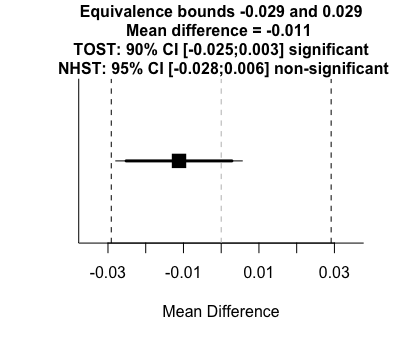
\includegraphics[width=0.5\linewidth]{plots/french_eng_tost}
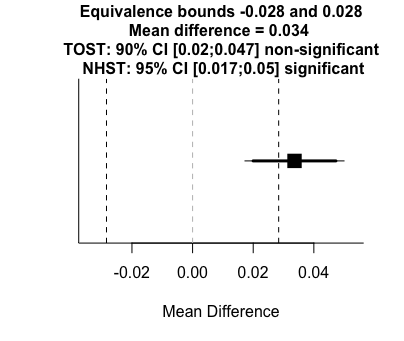
\includegraphics[width=0.5\linewidth]{plots/french_span_tost}

\hypertarget{references}{%
\subsection{References}\label{references}}

\begingroup
\setlength{\parindent}{-0.5in}
\setlength{\leftskip}{0.5in}
\phantom{.}

\textcolor{white}{\\} \vspace{-0.5in}

\begin{tiny}
Brysbaert, M. (2020). Power considerations in bilingualism research: Time to step up our game. Bilingualism: Language and Cognition, 1–6. 

Lakens, D. (2017). Equivalence Tests: A Practical Primer for t Tests, Correlations, and Meta-Analyses. Social Psychological and Personality Science, 8(4), 355–362. 

Lemhfer, K., \& Broersma, M. (2012). Introducing LexTALE: A quick and valid Lexical Test for Advanced Learners of English. Behavior Research Methods, 44(2), 325–343. 

Llama, R., \& Cardoso, W. (2018). Revisiting (Non-)Native Influence in VOT Production: Insights from Advanced L3 Spanish. Languages, 3(3), 30. 

Llama, R., Cardoso, W., \& Collins, L. (2010). The influence of language distance and language status on the acquisition of L3 phonology. International Journal of Multilingualism, 7(1), 39–57. 

St\"{o}lten, K., Abrahamsson, N., \& Hyltenstam, K. (2015). EFFECTS OF AGE AND SPEAKING RATE ON VOICE ONSET TIME: The Production of Voiceless Stops by Near-Native L2 Speakers. Studies in Second Language Acquisition, 37(1), 71–100.

Wrembel, M. (2011). Cross-linguistic Influence in Third Language Acquisition of Voice Onset Time. Proceedings of the 17th International Congress of Phonetic Sciences, 2157–2160.
\end{tiny}

\endgroup

\end{document}
